\chapter{Prototype simulations and desing}
\chaptermark{Prototype simulations and desing}
\cleardoublepage
\minitoc
\section{Introduction}
\begin{refsection}
	\label{ch3:Introduction}
	First the requirements for will be
	Then
	Lastly
	\section{Taille de la page}
	textwidth in cm: \printinunitsof{cm}\prntlen{\textwidth}
	\section{ESS requirements}
	\begin{figure}[ht]
	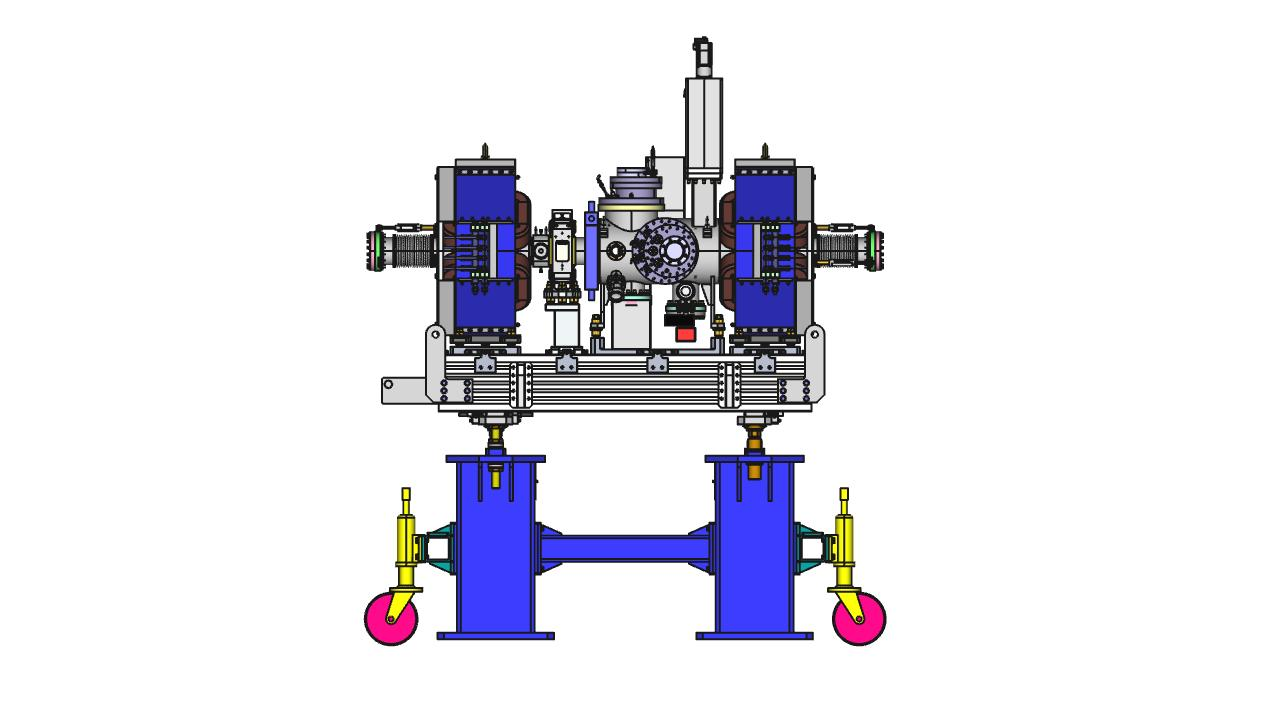
\includegraphics[width=\textwidth]{03_Prototype/figures/00_fig/fig007_LWU.jpeg}
	\caption[Typical mass stopping power plot]{Typical mass stopping power plot.}
	\label{chap3:maxwell_gas_log1}
\end{figure}

	\section{Electromagnetic fields simulations}

	\begin{align}
		 & \overrightarrow{\nabla} \cdot \overrightarrow{E} = \frac{\rho}{\epsilon_{0}}                                            \\
		 & \overrightarrow{\nabla} \times \overrightarrow{E} = - \frac{\partial \overrightarrow{B}}{\partial t}                    \\
		 & \overrightarrow{\nabla} \cdot \overrightarrow{B} = 0                                                                    \\
		 & \overrightarrow{\nabla} \times \overrightarrow{B} = \overrightarrow{J} + \frac{\partial \overrightarrow{E}}{\partial t}
	\end{align}

	\section{Extraction field}
	\subsection{Maxwell equations at steady state}
	\subsection{Solving poisson equation}

	\begin{align}
		 & f(x+h) = f(x)+hf^{\prime}(x)
		+\frac{h^2}{2}f^{\prime\prime}(x)+\frac{h^3}{6}f^{\prime\prime\prime}(x) + O(h^{4}) \\
		 & f(x-h) = f(x)-hf^{\prime}(x)
		+\frac{h^2}{2}f^{\prime\prime}(x)-\frac{h^3}{6}f^{\prime\prime\prime}(x) + O(h^{4})
	\end{align}

	\begin{equation}
		f^{\prime\prime}(x) = \frac{f(x+h) + f(x-h) - 2f(x)}{h^{2}} + O(h^{2})
	\end{equation}

	\begin{equation}
		\begin{split}
			h^{2}f^{\prime\prime}(x,y)&= f(x+h,y) + f(x-h,y) \\
			&+ f(x,y+h) + f(x,y-h) \\
			&- 4f(x)+ O(h^{2})
		\end{split}
	\end{equation}

	%\subsection{Finite Elements Method}
	\subsection{COMSOL}
	COMSOL\cite{comsol2018} is a proprietary software.\cite{comsolacdc2018}
	The user defines a geometry.
	Then the geometry is discretize
	\begin{figure}[ht]
	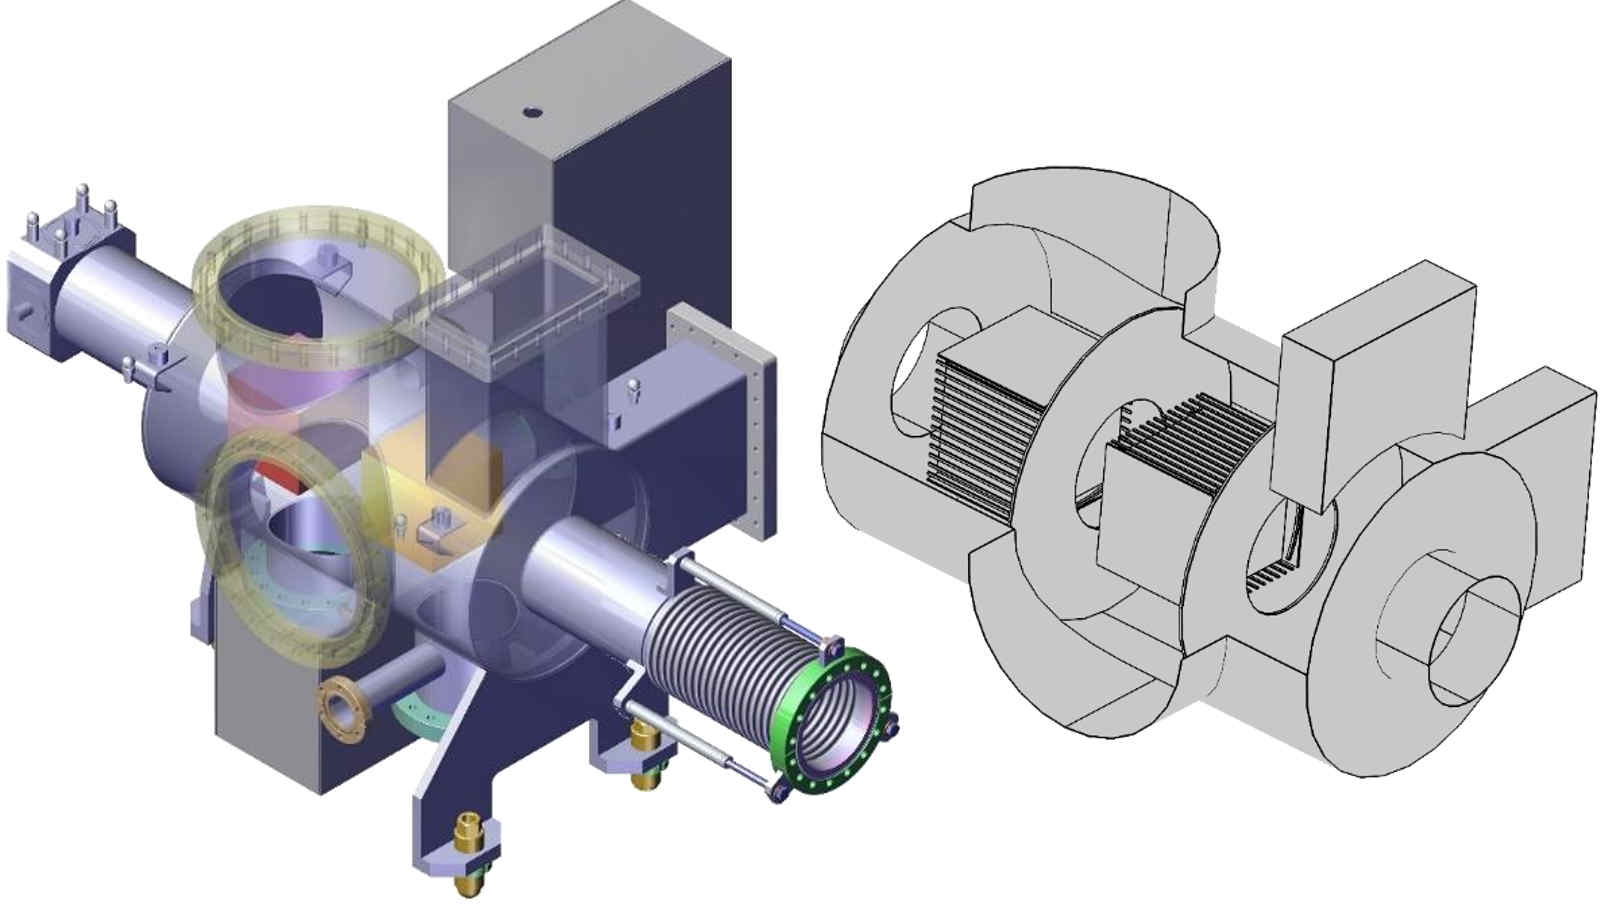
\includegraphics[width=\textwidth]{03_Prototype/figures/00_fig/fig003_COMSOL_LWU.jpeg}
	\caption[Typical mass stopping power plot]{Typical mass stopping power plot.}
	\label{chap3:maxwell_gas_log1}
\end{figure}


	\begin{figure}[ht]
	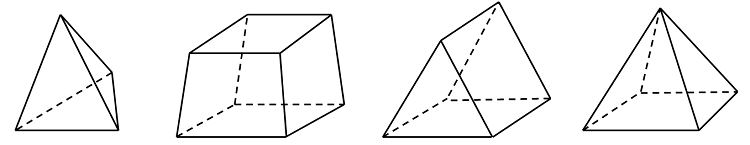
\includegraphics[width=\textwidth]{03_Prototype/figures/00_fig/fig006_COMSOL_meshing_elements.png}
	\caption[3D Mesh elements included in COMSOL]{Mesh elements included in COMSOL software. COMSOL uses tetrahedral elements by default to mesh a 3D geometry.}
	\label{chap3:maxwell_gas_log1}
\end{figure}


	\cite{cststudio2018}\cite{ansys2018}\cite{couloumb2018}
	\subsection{Criteria}
	\begin{figure}[ht]
	\includesvg[width=\textwidth]{03_Prototype/figures/00_fig/figure008_lorentz_evsp}
	\caption[Typical mass stopping power plot]{Typical mass stopping power plot.}
	\label{chap3:maxwell_gas_log1}
\end{figure}


	\subsection{IPM geometry}
	\subsection{IPM position and cross interaction}
	\subsection{Grid}
	\subsection{Field corrections}
	\subsection{IPM polarity}
	\section{Particle through matter}
	%TODO: Finir
	The interactions of particles with matter are an important aspect of nuclear or particle detection\cite[]{Leo1994, Knoll2010}.
	A particle loses energy when it passes through a medium.
	The physical process behind the energy transfer mainly depends on the characteristics of the particle.
	These topics has been studied and improved over the last century.
	It often combines complicated theoretical laws with approximations or empirical models.
	This topic is very wide, hence only the meaningful processes that are related to the IPMs will be described in the following sections.

	\subsection{Interraction of heavy charged particles with matter}
	%TODO: Finir
	For heavy charged particles, the main interaction is due to electromagnetic interactions of the incident particle with the orbiting electrons of the medium.
	A particle is considered heavy if its mass is far higher than the mass of an electron.
	The incident particle will transfer its energy to an electron of the medium at each electronic collision.
	The maximum transfer energy for one collision is given by the following equation:
	\begin{equation}
		T_{max} = \frac{2 m_{e} \beta^{2} \gamma^{2}}{1 + \frac{2 \gamma m_{e} }{M} + \left( \frac{m_{e}}{M} \right)^{2}}
	\end{equation}
	Where \(M\) is the mass of the incident particle and \(m_{e}\) is the mass of electron.

	The average linear stopping power is given equation\cite[]{Bethe1930} \cite[p. 446]{Tanabashi2018}
	\begin{equation}
		- \bigg \langle \frac{dE}{dx} \bigg \rangle =K \rho \frac{Z}{A} \frac{z^{2}}{\beta^{2}} \left[\frac{1}{2} ln \left(\frac{2 m_{e} \beta^{2} \gamma^{2} T_{max}}{I^{2}} \right) - \beta^{2} - \frac{\delta(\beta \gamma)}{2} - \frac{C}{Z} \right]
	\end{equation}
	The K constant is completely independant to the incident particle or the medium.

	Terms related to the medium, \(Z\) atomic number, \(A\) mass number, \(I\) mean excitation energy and \(\rho \) the medium density.
	One can see that the ratio \(Z/A\) is around \(0.5\).
	Usally is

	The terms related to the incident particle with \(\gamma\) \(\beta\) \(z\)

	Nevertheless the Bethe equation still quite precise for particle between

	The Fig. \ref{chap3:bethe1} shows

	\begin{figure}[ht]
	\includesvg[width=\textwidth]{03_Prototype/figures/00_fig/fig001_bethe_2}
	\caption[Typical mass stopping power plot for protons]{Typical mass stopping power plot for protons. Here the mass stopping is plotted for proton in hydrogen and nitrogen.The calculation was done with respect to the Bethe formula and has been crosschecked with NIST PSTAR table which contains both computed and experimental values \cite{Seltzer1993}. The Bethe equation gives between \(0.2\ <\ \beta\gamma\ <\ 100\). However at lower and higher energies the Bethe formula is no more reliable.}
	\label{chap3:bethe1}
\end{figure}


	\subsection{Electron ion pairs production}
	%TODO: Finish
	The mean linear stopping power.

	\cite[]{Weiss1955}
	\cite[]{Bichsel1979}
	\begin{equation}
		N_{electrons}= \frac{\big \langle \frac{dE}{dx} \big \rangle}{W_{n}} dx
	\end{equation}

	\begin{table}[ht]
	\centering
	\caption[W values for severals gases]
	{W values for severals gases.}
	\label{}
	\begin{tabular}{llr}
		\toprule
		Gas       & Description & Price (\$) \\
		\midrule
		Gnat      & per gram    & 13.65      \\
		          & each        & 0.01       \\
		Gnu       & stuffed     & 92.50      \\
		Emu       & stuffed     & 33.33      \\
		Armadillo & frozen      & 8.99       \\
		\bottomrule
	\end{tabular}
\end{table}

	The W value is usually measured

	\subsection{Case of a mixture}
	%TODO: Finish
	When the medium is a mixture of several compounds then it is necessary to calculate the mean stopping power for each of them with respect to their mass proportions:
	\begin{equation}
		N_{total}= \sum_{n= First}^{Last} N_{compound\ n}= \sum_{n= First}^{Last} w_{n} \frac{\big \langle \frac{dE}{dx}\left(\rho_{n},I_{n},A_{n},Z_{n}\right) \big \rangle}{W_{n}} dx
	\end{equation}
	The calculation can be done for each single element or for each molecule in the compound.
	However the second computation is preferable since the I and W values are in general smaller.
	\subsection{Calculation}
	\begin{table}[ht]
	\centering
	\caption[Expected residual vacuum gas in the cold part of ESS Linac, provided by ESS vacuum group]
	{Expected residual vacuum gas in the cold part of ESS Linac, provided by ESS vacuum group.}
	\label{chap3:ess_vacuum_gas}
	\begin{tabular}{llll}
		\toprule
		Gas        & Mass percentage (\(\%)\) & $p_{i}$ (\(\mathrm{mbar}\)) & $\rho_{i}$ $(\mathrm{g/cm^{3}}$) \\
		\midrule
		\(H_{2}\)  & \(79\)          & \(7.9 10^{-10}\)   & \(6.52\cdot
		10^{-17}\)                                                                \\
		\(CO\)     & \(10\)          & \(1.0 10^{-10}\)   & \(1.15\cdot
		10^{-16}\)                                                                \\
		\(CO_{2}\) & \(10\)          & \(1.0 10^{-10}\)   & \(1.8\cdot
		10^{-16}\)                                                                \\
		\(N_{2}\)  & \(1\)           & \(1 10^{-11}\)     & \(1.14\cdot
		10^{-17}\)                                                                \\
		\bottomrule
	\end{tabular}
\end{table}
	\subsection{Simulations}
	\subsection{Limits}

	\subsection{Interraction of light charged particles in matter}
	%TODO: Finish
	If the incident particle
	In case of the incident particle is an electron the
	So the Bethe Bloch should be corrected for electron.\cite{Rieke1972}
	\begin{equation}
		- \bigg \langle \frac{dE}{dx} \bigg \rangle = \frac{1}{2} K \rho \frac{Z}{A} \frac{1}{\beta^{2}} \left[ln \left(\frac{2 m_{e} \beta^{2} \gamma^{2}}{2I^{2}} \right) + (1 - \beta^{2})\right]
	\end{equation}
	\subsection{Initial momentum}
	\begin{figure}[ht]
	\includesvg[width=\textwidth]{03_Prototype/figures/00_fig/fig002_maxwell_gas_log}
	\caption[Typical mass stopping power plot]{Typical mass stopping power plot.}
	\label{chap3:maxwell_gas_log1}
\end{figure}

	\section{Readout simulations}
	\subsection{Ramo-Schoktley theorem}
	\cite[]{Ramo_1939}\cite[]{Shockley_1938}\cite[]{Cavalleri1971}\cite[]{Jen1941}
	\subsection{Strips based readout}
	\subsection{MCP based readout}
	\subsubsection{Micro Channel Plate}
	\subsubsection{MCP models}
	\subsection{Silicon based readout}
	\begin{figure}[ht]
	\includesvg[width=\textwidth]{03_Prototype/figures/00_fig/fig004_ion_si_deposit}
	\caption[Typical mass stopping power plot]{Typical mass stopping power plot.}
	\label{chap3:bethe1}
\end{figure}

	\begin{figure}[ht]
	\includesvg[width=\textwidth]{03_Prototype/figures/00_fig/fig005_ion_si_range}
	\caption[Typical mass stopping power plot]{Typical mass stopping power plot.}
	\label{chap3:bethe1}
\end{figure}


	\subsubsection{TimePix3}
	\subsubsection{Simulations}
	\subsubsection{Tests at IRMA}

	\section{Summary}
	\label{ch3:Summary}

	\cleardoublepage
	\section{Bibliography}
	\label{ch3:bib}
	\printbibliography[heading=subbibliography]
\end{refsection}